\chapter{Mechanical Structure and Envelope}
\label{chap:mse}

This subsystem is considered to be the foundation of the whole airship, given that it has to act as the pillar that withstands and holds all the other subsystems together. Aside from this structural requirements, it also includes the device that will be generating lift, which is in this case the same blimp. This adds to the picture additional light weight requirements, which consequences will be explained on this section.
\\ 
\\
The fact that we decided to use the ESRANGE blimp, rather than building our own due to the time constraint, has modified virtually every single requirement that was previously estimated in the preliminary calculations (refer to the \ac{PDR}). Therefore, one of the aspects that will be covered in this document are the updated requirements and constraints together with the view on the possible alternatives to overcome the problems that we are currently facing with the project. Nevertheless, the current design under construction will be also presented, however the reader should bear in mind that this are only guidelines to take the firsts steps, given that the design is not closed due to the uncertainty surrounding the final components to be used. 

\section{Functional and Technical Requirements}

This section will cover the updated requirements that are consequence of the choices taken during the evolution of the project. As it will be seen, obviously the functional requirements have not change, however the same cannot be said about the technical ones. 

\pagebreak

\subsection{Functional Requirements}

\begin{itemize}
\item The structure has to be stable aerodynamically
\item The structure has to act has a support for the solar cells and/or the payload
\item The lift has to be large enough to overcome the weight of the total system
\item The material of the balloon must have low diffusivity
\end{itemize}


\subsection{Technical Requirements}

The previous calculated/estimated parameters have been modified to fit the constraints imposed by the ESRANGE blimp. 

\begin{itemize}
\item Lenght = 4.88 m
\item Diameter = 1.89 m
\item Volume = 15 cubic m
\item Max. Lift Weight = 2.59 kg
\item Max. Lift Payload Weight = 0.5 kg
\item Max. Lift Structure Weight = 1 kg
\item Max. Lift Power System Weight = 1 kg
\end{itemize}

\noindent
Comparing the new available maximum lift weight provided by the blimp, it can be seen that the new total weight is half of the one that it was initially assumed on the \ac{PDR}. This entails that the weight budgets available for each of the subsystems had to be redistributed. For this system in particular, the consequence was a complete redesign of the structure, leaving the initial idea of a rigid structure completely out of place. The next section will explain how this design was redone with the corresponding suggested new structure components. 

%General introduction to the subsystem...

%\section{Functional and Technical Requirements}

%\textit{Will be added in the final version...}

\section{Critical Design}

As was mentioned in the \ac{PDR}, the initial mechanical design of the \ac{U-SPACE} project included the development of a blimp (envelope) that would then accommodate the solar panels of the \ac{EPS}, the cargo bay for the \ac{ITPU} and the propelling system of \ac{MCC}. An initial sketch of this concept is presented in figure \ref{fig:init}. 

\pagebreak

\begin{figure}[bht]
\centering
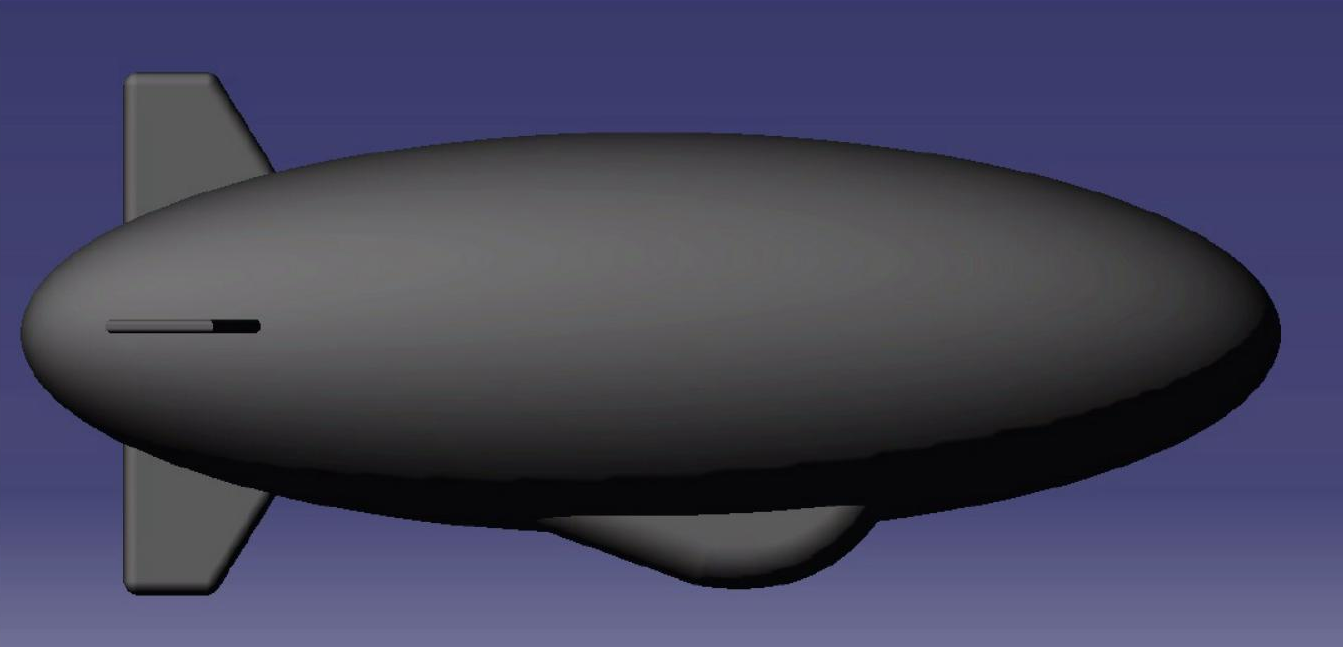
\includegraphics[scale=0.5]{figures/init.png}
\caption{Initial 3D sketch of the airship}
\label{fig:init}
\end{figure}

\noindent
This simplified view of the mechanical design shows that it included the total development of the envelope of the airship. The idea was to include the solar panels on the top, mounted on a wired mesh, with the cargo bay attached in the bottom together with the propelling system.
\\
\\
However, due to new developments in the project that included the introduction of an already built blimp (envelope), the focus of the mechanical design changed. The blimp to be used would be the TIF-250 (Tethered Aerostats), shown in figure \ref{fig:blimp}. This blimp has the capacity to lift a payload of about 2.5 kg, has a length of approximately 5 m and has a diameter (in the center) of about 1.9 m.

\vspace{1.0em}

\begin{figure}[bht]
\centering
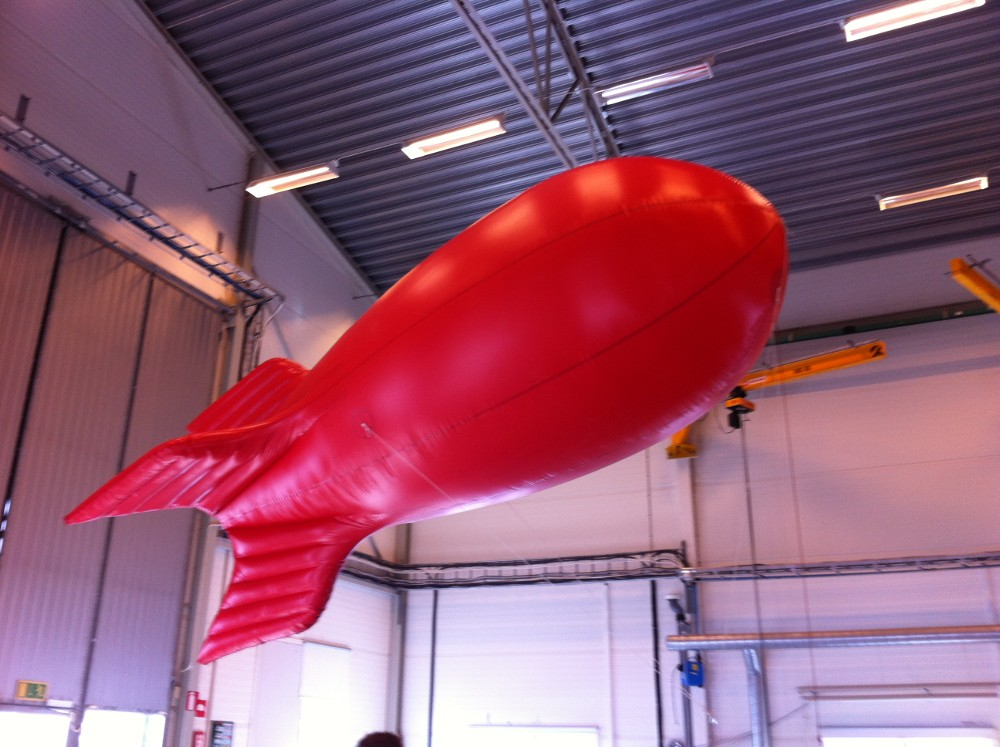
\includegraphics[width=\textwidth]{figures/blimp.jpg}
\caption{TIF - 250 Blimp}
\label{fig:blimp}
\end{figure}

\noindent
This blimp serves the purpose of the U-SPACE project very well, as its use would allow to focus only on the construction of the support for the power system, the cargo bay (for the payload) and the integration of the propelling system. However, because it is a ready-built blimp with a purpose different than the one envisioned, it is not as lightweight as might be needed. Nevertheless, an effort will be made to include light structures in the integration of all the other systems in this airship.

\subsection{Envelope}

As it was already stated, the blimp to be used is a ready-built one. This blimp is normally used to accurately measure the wind direction. Nevertheless it will have to fit the purpose of the U-SPACE project, due to the lack of time to build a new envelope. This way, the envelope is constituted by the blimp itself.  

\subsection{Cargo Bay}

The cargo bay is intended to accommodate both the payload and the electronics required for the purpose of the project. The main challenge in the construction of this cargo bay is the weight. It has to be lightweight (the total maximum weight of all the structures should be less than 1 kg) but at the same time rigid enough to resist some stress during the normal operation of the airship. To achieve this, balsa wood reinforced with carbon fibres was used. Figures of the expected final cargo bay design and of the current construction status are presented in figures \ref{fig:box} and \ref{fig:boxinit}, respectively. 

\begin{figure}[th!]
\centering
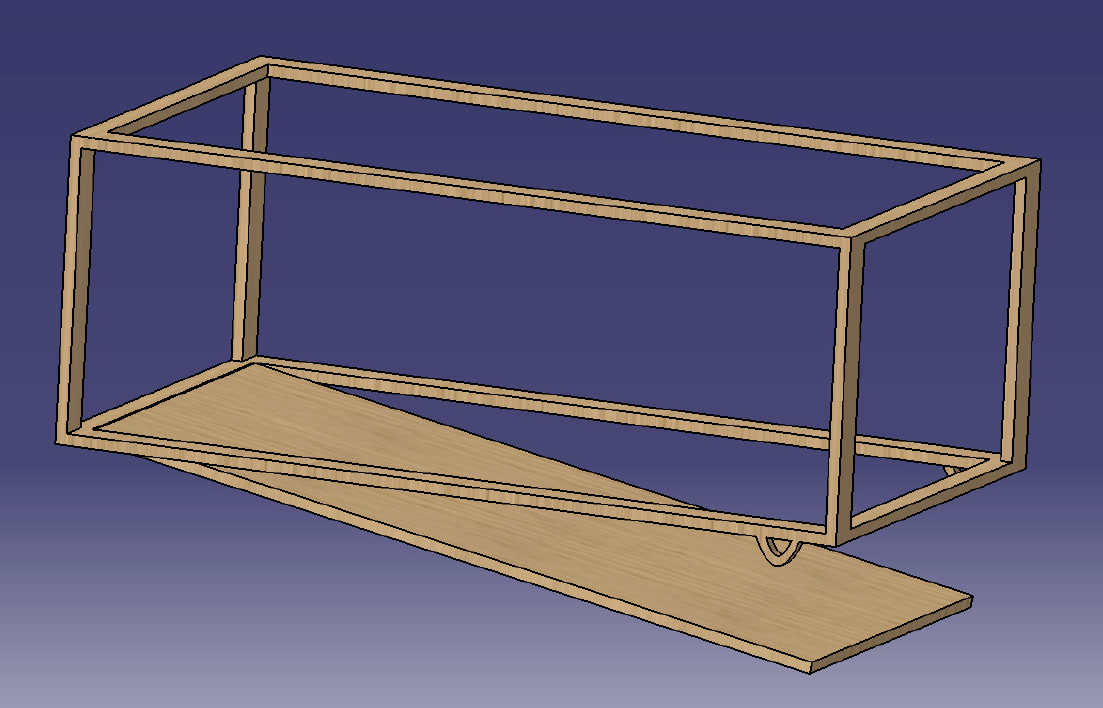
\includegraphics[scale=0.5]{figures/box.png}
\caption{3D sketch of the cargo bay} 
\label{fig:box}
\end{figure}

\begin{figure}[th!]
\centering
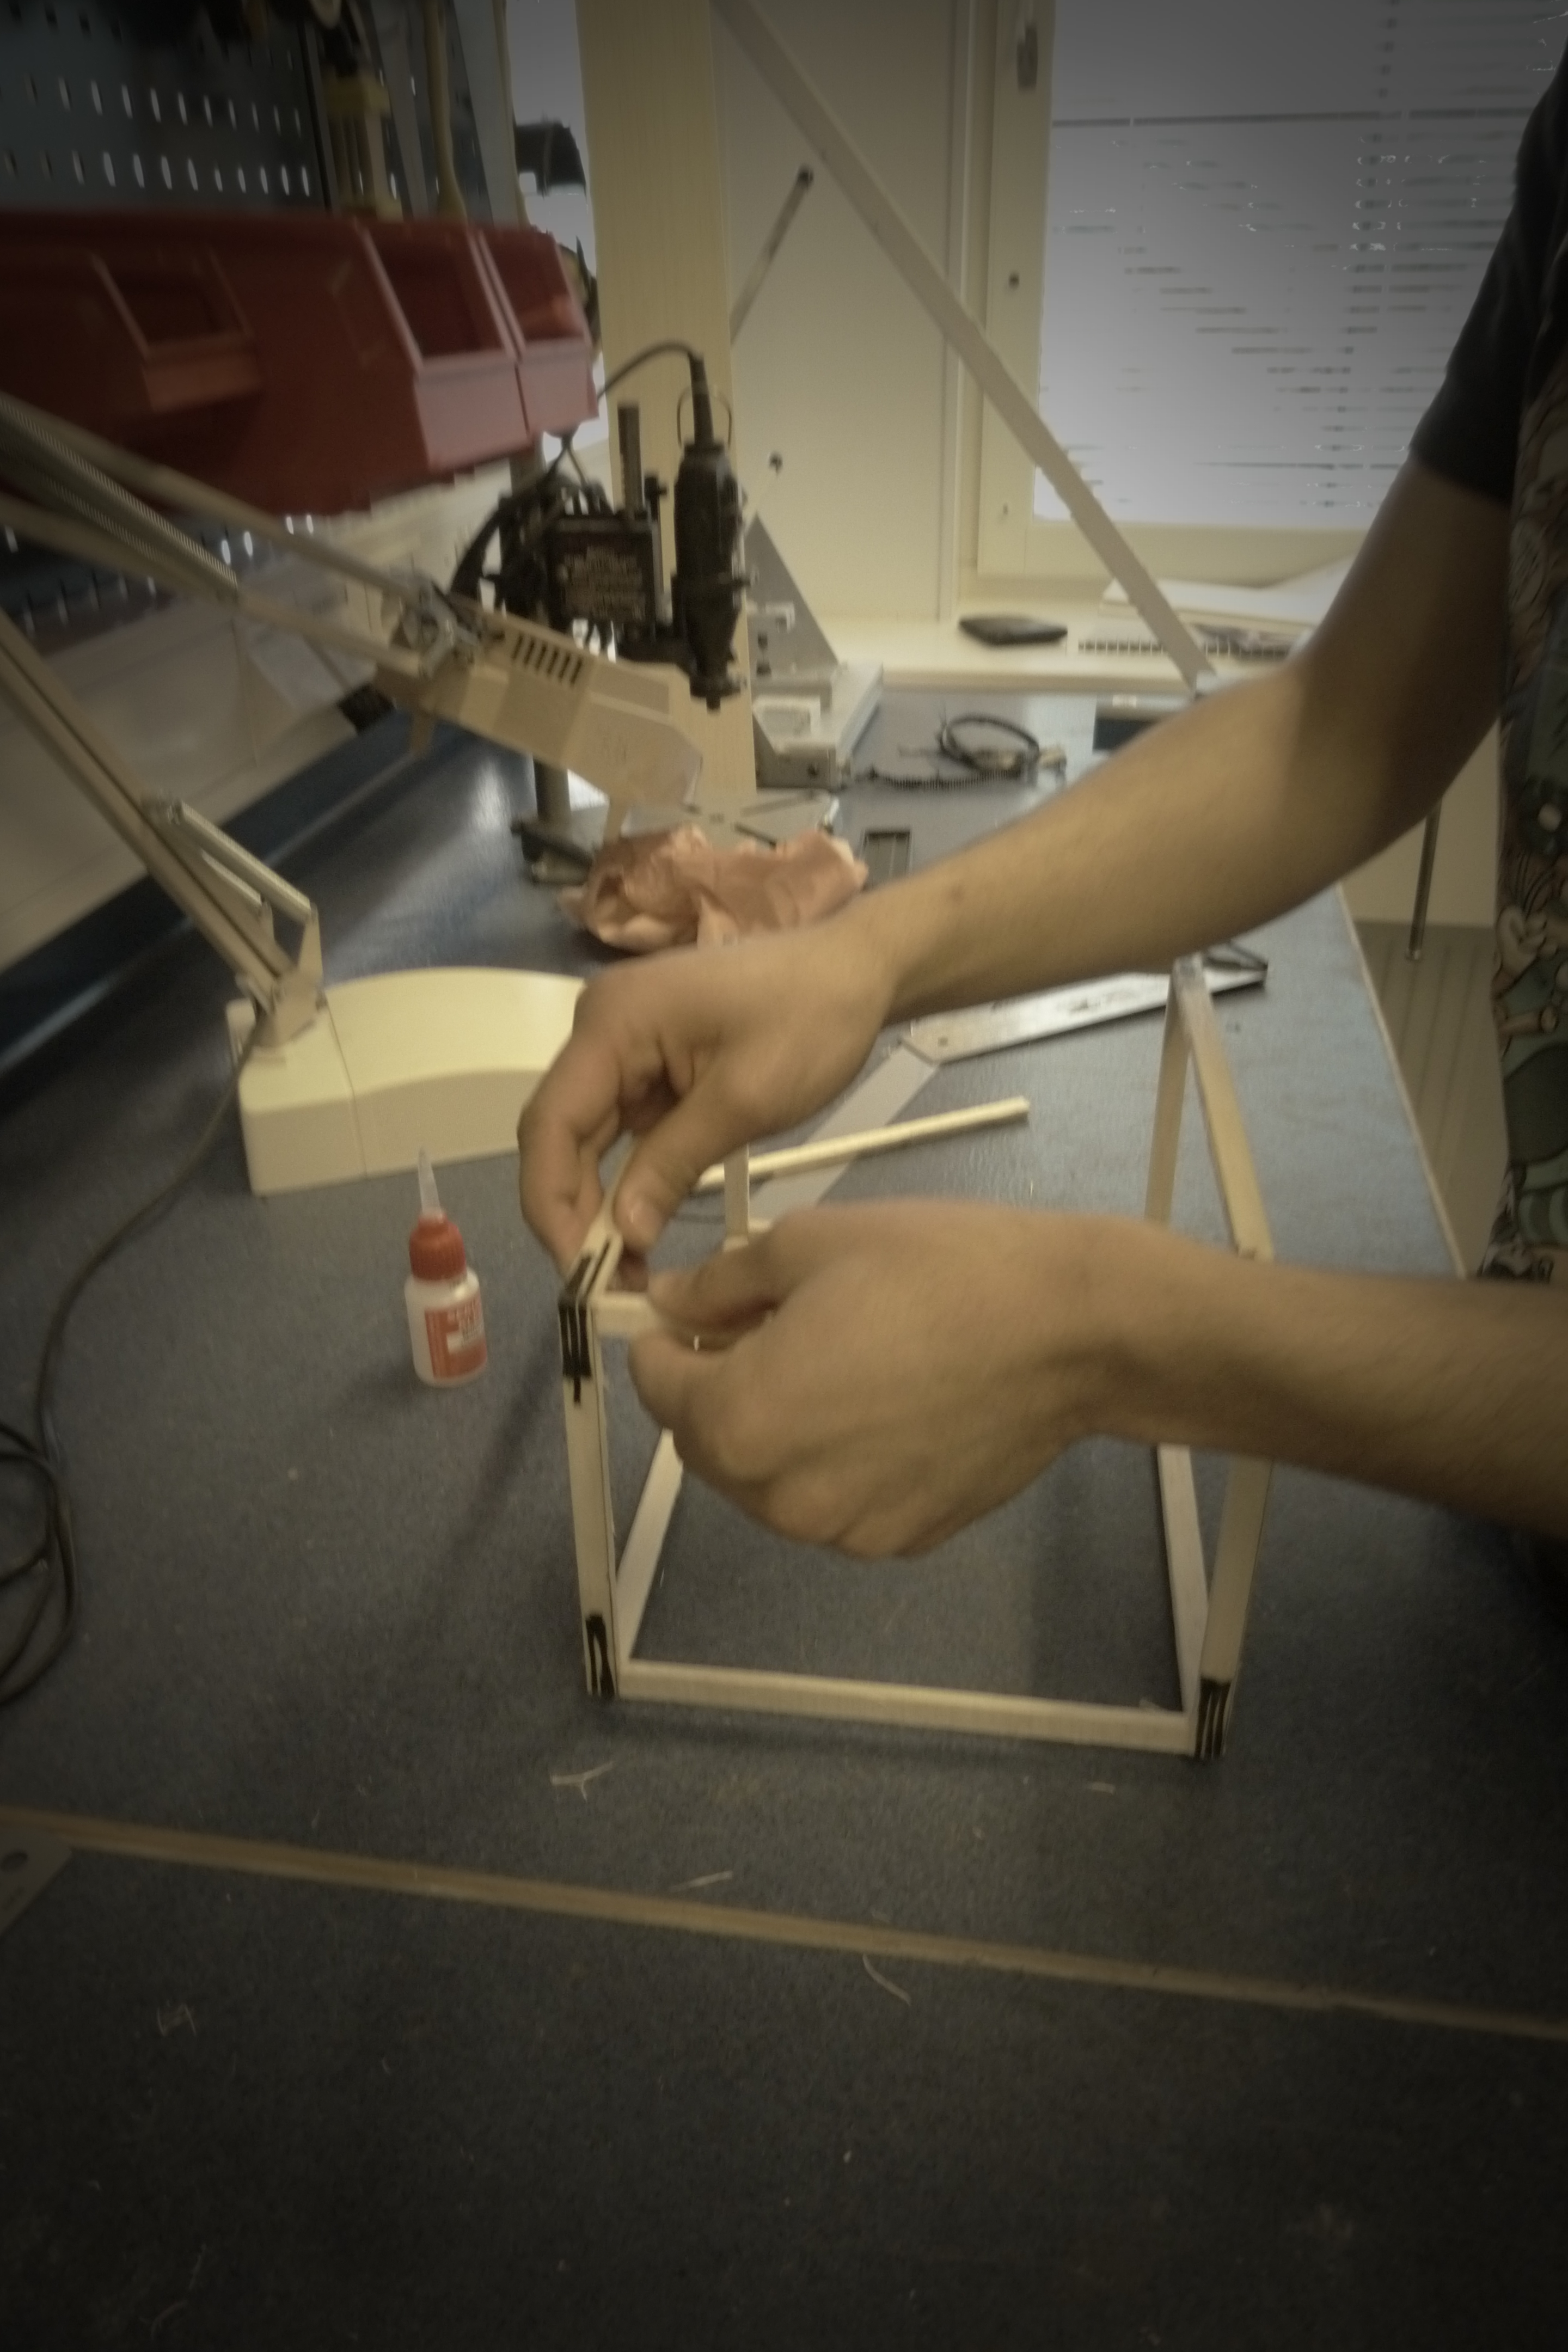
\includegraphics[scale=0.5]{figures/boxinit.jpg}
\caption{Initial construction phase of the cargo bay}
\label{fig:boxinit}
\end{figure}

\subsection{Power System}

The biggest challenge of this project is to accommodate the power system, taking into account the maximum lift weight and also the power requirements that consequently influence the solar panel quantity and weight. Because different solar panels are still under test, it is still not decided how they will be mounted on the blimp. Nevertheless, the idea is to use a lightweight wired mesh that serves as a support to the solar panels, which are attached to the wires with carbon fibre. This mesh will then be connected to the blimp making use of 3 bands that will round the blimp, distributing the weight along the envelope. These bands will be made of fibre glass reinforced rubber tape. An idea of how the final product should look like is presented in figure \ref{fig:mesh}.

\pagebreak

\begin{figure}[bht]
\centering
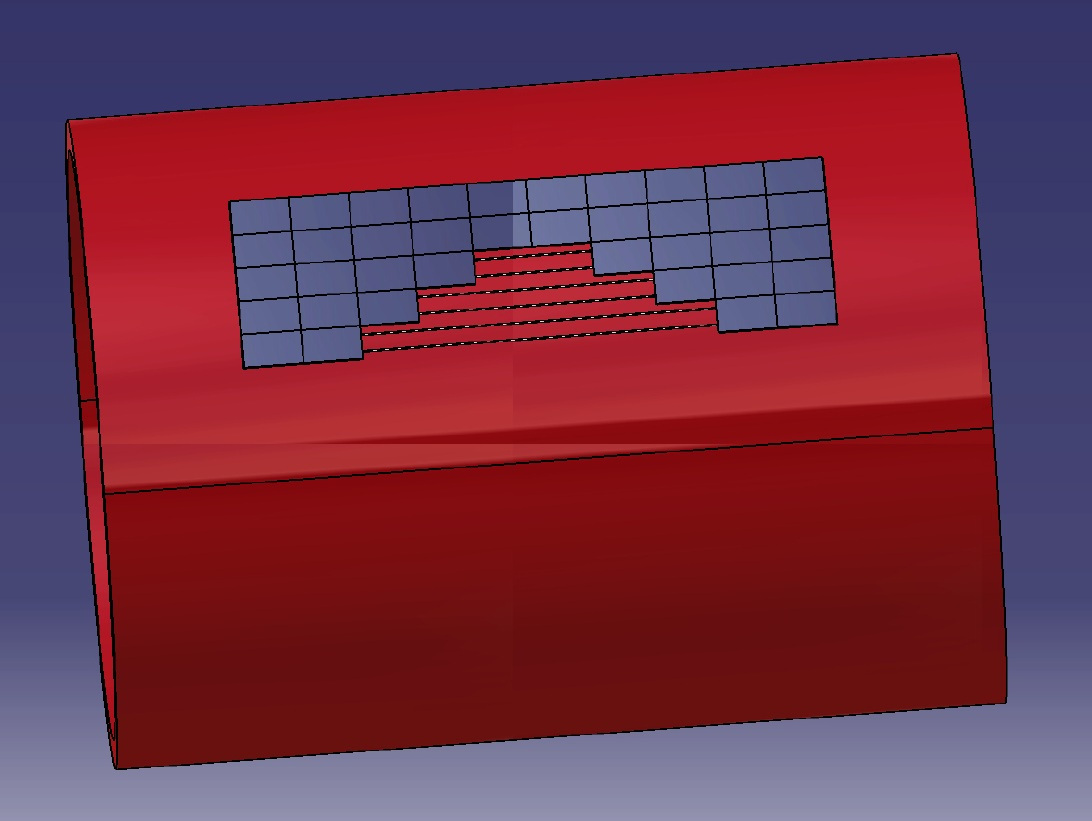
\includegraphics[scale=0.4]{figures/mesh.jpg}
\caption{3D sketch of the integration of the power system}
\label{fig:mesh}
\end{figure}

\subsection{Propelling System}

The propelling system is to be integrated in a carbon fibre rod mounted on the top of the cargo bay. The 2 motors will be attached at the ends of the rod, outside the influence of the envelope and free to achieve their maximum aerodynamic capabilities. A hand sketch of this principle is showed in figure \ref{fig:prop}.

\begin{figure}[h!]
\centering
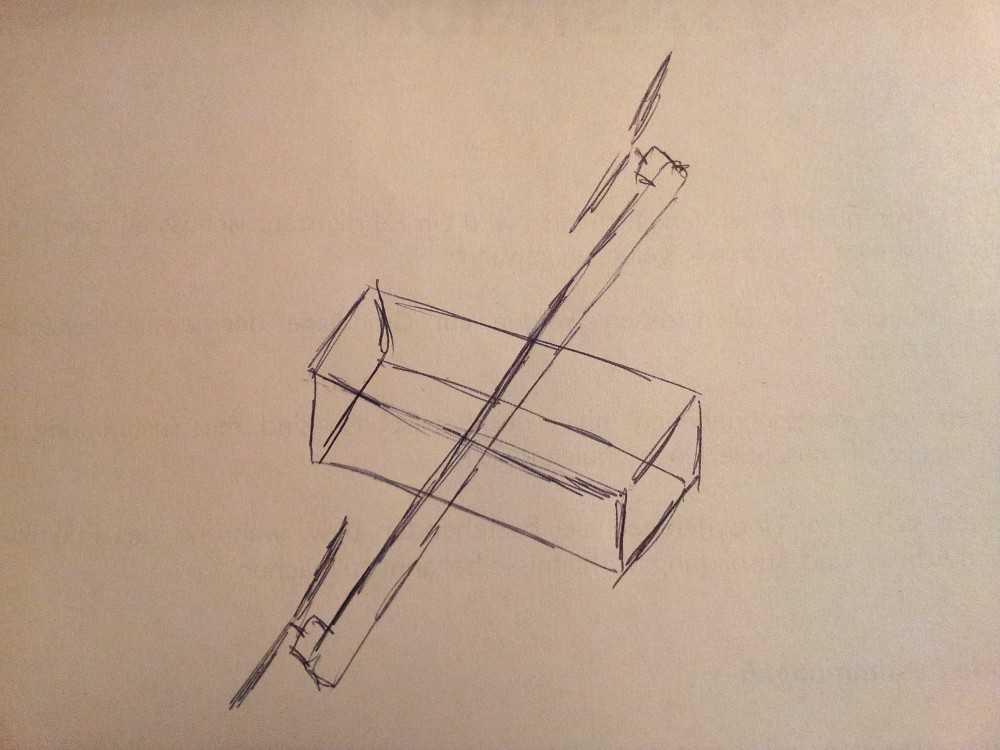
\includegraphics[scale = 0.3]{figures/prop.jpg}
\caption{Hand sketch of the integration of the propelling system}
\label{fig:prop}
\end{figure}

\section{Future Developments}

All the previously explained designs have to be built and tested. Conclusions have to be made and inputs from the other subsystems have to be taken into consideration. Only after a careful building of the different structures to accommodate all the required subsystems, it will be possible to check if the requirement of the maximum lift weight - the most important requirement - is achieved. For now, the 3D designs, the envisioned materials and previous experiences in the field give hope that this constraint will be surpassed.
\\
\\
The following steps should be to finish the construction of the cargo bay, accommodate the propelling system into it and then proceed with the construction of the wiring mesh and the consequent attachment of the solar panels.
%\section{Mechanical Interfaces}
%
%How does the MSE system interact with the other subsystems?
%
%\subsection{Mechanical Interface Control Drawing}
%
%Could not really find what this is and if we need it... Morten?
%
%\subsection{Accommodation Requirements}
%
%Same here...
%
%\section{Physical Properties}
%
%E.g. mass in launch configuration...
%
%\section{Structural and Mechanisms Analysis}
%
%This involves things like dynamic analysis and stress analysis, but as we didn't really do this, just briefly comment on it...
%
%\section{Mounting Attachments}
%
%Not sure what they mean with this... Attachment concept and foot pattern?